\documentclass[12pt, oneside]{article}   	% use "amsart" instead of "article" for AMSLaTeX format
\usepackage[margin=1in]{geometry}                		% See geometry.pdf to learn the layout options. There are lots.
\geometry{letterpaper}                   		% ... or a4paper or a5paper or ... 
%\geometry{landscape}                		% Activate for for rotated page geometry
%\usepackage[parfill]{parskip}    		% Activate to begin paragraphs with an empty line rather than an indent
\usepackage{float}
\usepackage{graphicx}				% Use pdf, png, jpg, or eps§ with pdflatex; use eps in DVI mode
%\usepackage{amsmath}
%\usepackage{CJK}	% convert eps --> pdf in pdflatex		
\usepackage{achemso}
\usepackage{amssymb}
\usepackage{indentfirst}
\usepackage{url}


\title{Interim Report of Predicting Chemical Properties Using Machine Learning Methods}
\author{Andrew IDs: ccollin1, haichenl, zhonghal}
%\date{}							% Activate to display a given date or no date

\begin{document}
\maketitle

\begin{abstract}
We have obtained 12 sets of data through quantum mechanic density functional theory calculation, each set contains 557 different samples (molecular structures). Based on chemical compositions and properties of these structures, we have developed, so far, 6 types of feature vectors for implementing machine learning algorithms. Linear Ridge regression, SVM (with Gaussian and Laplacian kernels), k-NN and decision tree methods have been performed on all types of feature vectors. To some extent, reasonable agreement with quantum mechanical calculations has been achieved.    
\end{abstract}
\section{Introduction}
%\subsection{}
\noindent Quantum mechanics allows us to predict chemical compounds' properties to a very high accuracy, given that we are able to solve certain nonlinear ill-conditioned partial differential equations. Density Functional Theory (DFT) and \textit{ab initio} theory are two common types of methods to solve quantum differential equations; they possess the powerful advantage that in principle they are applicable to every type of chemical compounds. DFT has been used extensively for predicting chemical properties as a proper compromise between accurate (yet extremely expensive, typically $O(n^7)$ to $O(n!)$ in both time and space) \textit{ab initio} methods and cheap ($O(n^2)$ but can only achieve qualitative accuracy) Semi-Empirical Quantum Chemistry (SEQC) methods. Unfortunately, DFT methods still scale at least as $O(n^4)$ in both time and space, which means that they can only be applied to chemicals that have on the order of hundreds of atoms. Unfortunately, often in chemistry research, people deal with chemicals that consist of thousands of atoms every day (or hundreds of thousands in the case of biochemistry). The main benefit of a machine learning approach to doing these calculations would be that it could potentially be much faster and still retain the same level of accuracy as slower DFT calculations.

Recent studies show that a variety of machine learning regression models can be employed to predict chemical properties. Instead of solving partial differential equations directly, machine learning models try to predict chemical properties from "chemical similarities". From a chemist's point of view, chemicals are made of only a small set of structural building blocks, the properties of which have been thoroughly studied. Molecules consisted of similar building blocks are very likely to share similar chemical properties. Therefore, it is reasonable to train our machine learning models with features come from chemicals made of only a few building blocks, then use these models to predict properties of chemicals that constitute a great number of building blocks. An analogy is to train a spam filter with e-mails that have only a few sentences, and hope that this filter can classify not only short e-mails but also long e-mails that have similar sentences as our training examples do. Unlike quantum mechanical models which are considered "universal", our models will be, for sure, only applicable to a subset of chemicals, but that is just the inevitable trade-off between accuracy and generality. \\

Philosophically, our feature engineering part is highly related with our chemistry knowledge about our target molecules. It is expected that we can extract chemically informative characteristics of every molecule in both training stage and test stage. We have implemented 6 different ways to transform structural features of all the sample molecules into feature vectors. On the other hand, our training labels are supposed to be generated through quantum mechanical calculations, which require a solid understanding of the physics behind. Right now we basically treat this type of calculation as a black box, but in quantum chemistry there exist ways about how to reformulate complicated partial differential equations into simple ones--that is what most of the SEQC methods do, and we are planning to take advantage of this point in feature engineering. Specifically, we are interested in establishing regression models of the energies of highest occupied molecular orbital (HOMO), lowest unoccupied molecular orbital (LUMO), and band gap. These 3 properties are of great chemistry/physics interests both theoretically and experimentally, since they are directly related with molecules' spectroscopic behaviors. In case of machine learning models, five different types of algorithms, namely linear ridge regression, SVM (with Gaussian and Laplacian kernels), k-Nearest Neighbors, and decision tree, have been tested so far, both to evaluate the quality of our feature engineering and the suitableness of the machine learning models for our problem. We will present corresponding training/testing errors of combinations of different feature vectors and machine learning models later in this report. \\

\section{Data and Feature Vectors}


\noindent Right now we have 557 characteristic polymeric systems (chemicals that are built from repeated units, like plastic/rubber/Nylon) in our tentative training set. These systems are made up from 4 different major building blocks, (phenyl, furan, vinyl, and acetylene), and 5 minor building blocks, (Hydrogen, methyl, hydroxyl, methoxy, and carbenyl). Combinations of major/minor building blocks give us $\approx 100$ full building blocks which are then used to construct the 557 polymeric systems. Ideally, in the near future we will include an additional 1100 polymeric systems, but the corresponding DFT calculations still require about 2 weeks to finish. Quantum chemistry software package \textit{Gaussian} \cite{gaussian} is applied to compute HOMO, LUMO and band gap at three different DFT levels, namely B3LYP, CAM-B3LYP, and M06HF. These 3 theories have been widely tested in chemical research, and they lead to slightly different numerical results. In addition, each of these method defines an energetically favored geometrical structure for each of the molecules; these structures are slightly different, and it is reasonable to think that each of them contains some information. Along with the initial non-optimized geometrical structure, we have 4 types of structures; combining with the aforementioned 3 DFT theories, we have essentially obtained 12 data sets that contain slightly different information. \\


The following part shows feature engineering works we have done so far, i.e. how we extract 6 types of feature vectors from each structure:

\begin{enumerate}
\item \textbf{Null}: An empty list that serves as the worst result to compare against. This feature vector also is used to compare the amount of error that is contained implicitly in each of the different data sets.

\item \textbf{Binary}: It creates a simple boolean feature vector based on whether or not a building block exists in the structure. Mostly speaking, we only consider the existence of aryl-group and r-group. For example, a structure named as $``4aa"$ will form a vector $``4aa" \to [0, 0, 1, 0, 0, 0, 1, 0, 0, 0, 0, 0, 1, 0, 0, 0, 0]$

\item \textbf{Flip Binary}: This is similar to the binary feature vector, except that for each aryl group that appears in the structure, it takes into account whether or not the ring was rotated 180 along the connecting bond between the two units. When dealing with conjugated systems, like we have, the rotations can be a significant effect. This vector takes that into account by adding an extra binary feature for each link in the chain.

\item \textbf{Decay}: This feature vector makes the approximation that the relation between all of the atoms/structures within the molecule have some sort of a intrinsic decay, (atoms infinitely far apart should not influence each other). For this, the first aryl group in the chain is considered the zero point (influence of 1), and all the subsequent aryl groups influences are defined by a decay function $\sum_{i} (Ad_{i}^{-H})^{p}$, where $A$, $H$, $p$ are constant factors to determine rate of decay, $d_{i}$ is the distance from the $i$th group. This feature also has the added benefit that it has $O(1)$ space requirements compared to the normal binary feature vector which is $O(N)$ where $N$ is the number of aryl groups.

\item \textbf{Centered Decay}: This feature vector takes the same approach as the decay feature vector with the addition that it does the decay from the center of the structure using a radial distance.

\item \textbf{Signed Centered Decay}: This works similar to the centered decay feature vector with the addition that it takes into account the side of the center that the rings are on instead of just looking at the magnitude of the distance.

\end{enumerate}

To take into account the different datasets, an extra bit of meta data is attached to the end of each of the feature vectors. The first part is a four component boolean vector that indicates which method was used to optimize the structure (either ``non-optimized", ``B3LYP", ``CAM-B3LYP", or ``M06HF"). The second part consists of three boolean values that indicate the final DFT method that was used to calculate the molecular properties (``B3LYP", ``CAM-B3LYP", or ``M06HF"). Finally, all of the feature vectors then have an extra bias term added to the end.


\section{Machine Learning Algorithms and Current Results}
\noindent Key for distribution of work: Christopher Collins (CC), Haichen Li (HL), Zhonghao Luo (ZL) \\

We choose Python SciKit-Learn package\cite{scikit-learn} as our machine learning library, which already has various algorithms including linear ridge regression, SVM, k-NN, and regression tree readily available. We have implemented our own interface routines in order to fulfill our needs and to communicate with \textit{Gaussian} quantum chemistry package (CC designed and implemented the main framework, HL and ZL added modules that correspond to their own main focus).

Many of the machine learning methods used for this project require optimizing various hyper parameters. To do this, first, a reasonable value for each of the hyper parameters was selected, and then more values were added (both larger and smaller) on a logarithmic scale to get an overall view of which hyper parameters work the best.

To pick the best hyper parameters for each of the models, they all underwent two layers of k-folds cross validation (both layers were done with 10 folds each) (CC's work). The outer layer was used to set aside the test set, and the inner was used to cross validate for all of the hyper parameters in the models. The hyper parameters that produced the lowest errors in cross validation were then used on the test set to get the final results. The mean and standard deviations were then collected from these sets to produce a final error result. These results can be seen in Figures \ref{fig1}, \ref{fig2}, and \ref{fig3}.

\begin{figure}
\begin{center}
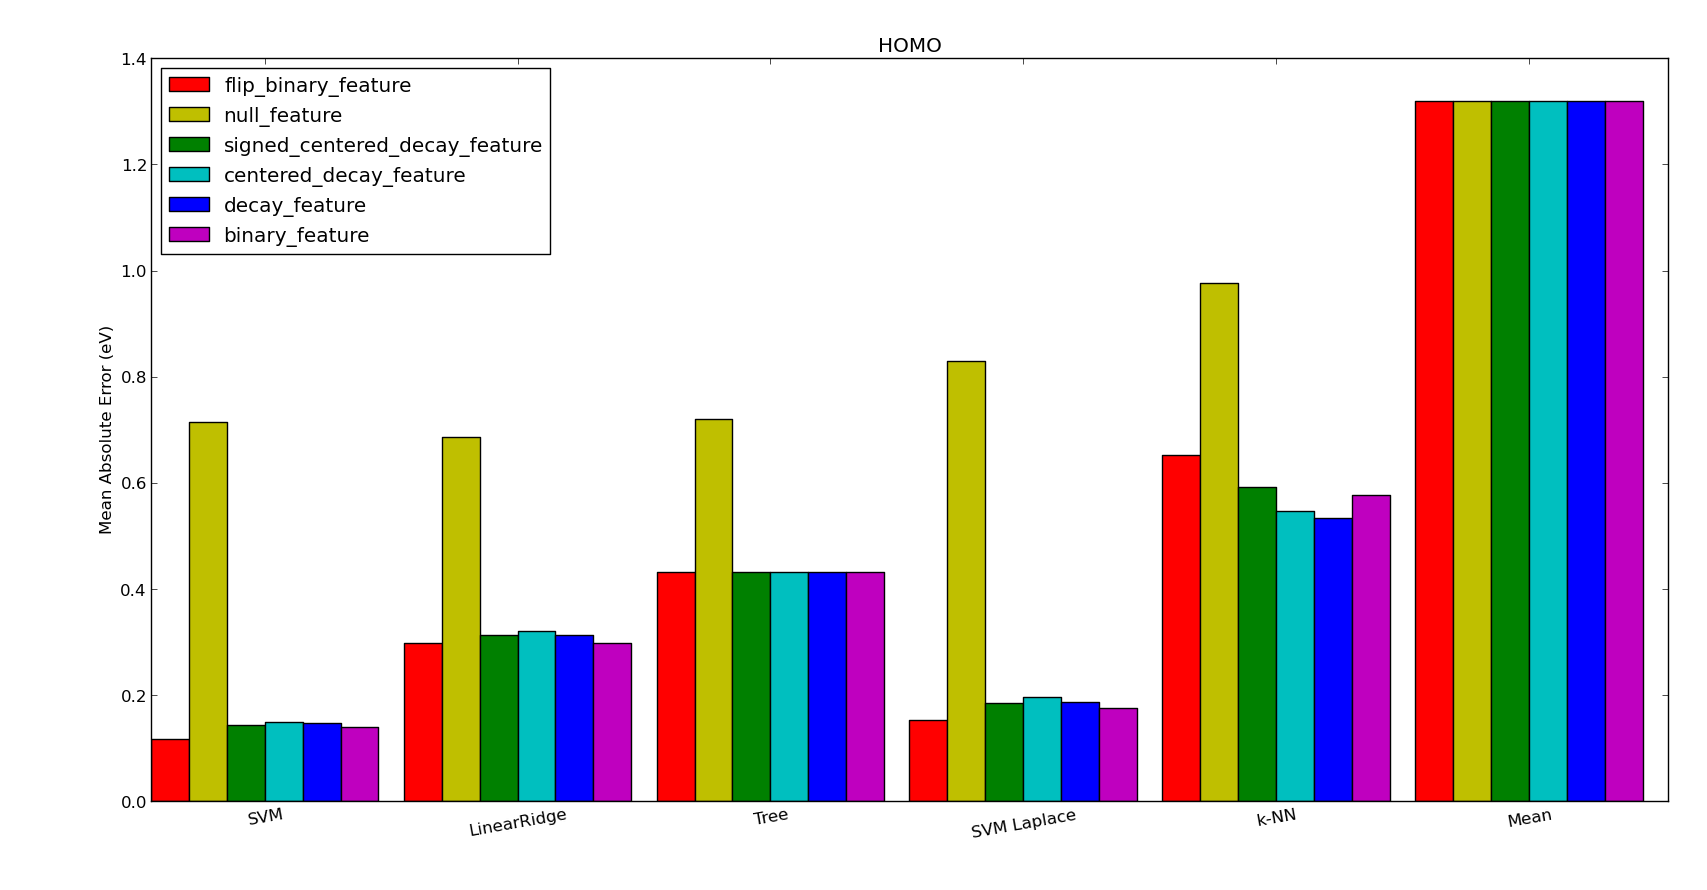
\includegraphics [width=1\textwidth]{homo.png}
\caption{Test error results for HOMO}\label{fig1}
\end{center}
\end{figure}

\begin{figure}
\begin{center}
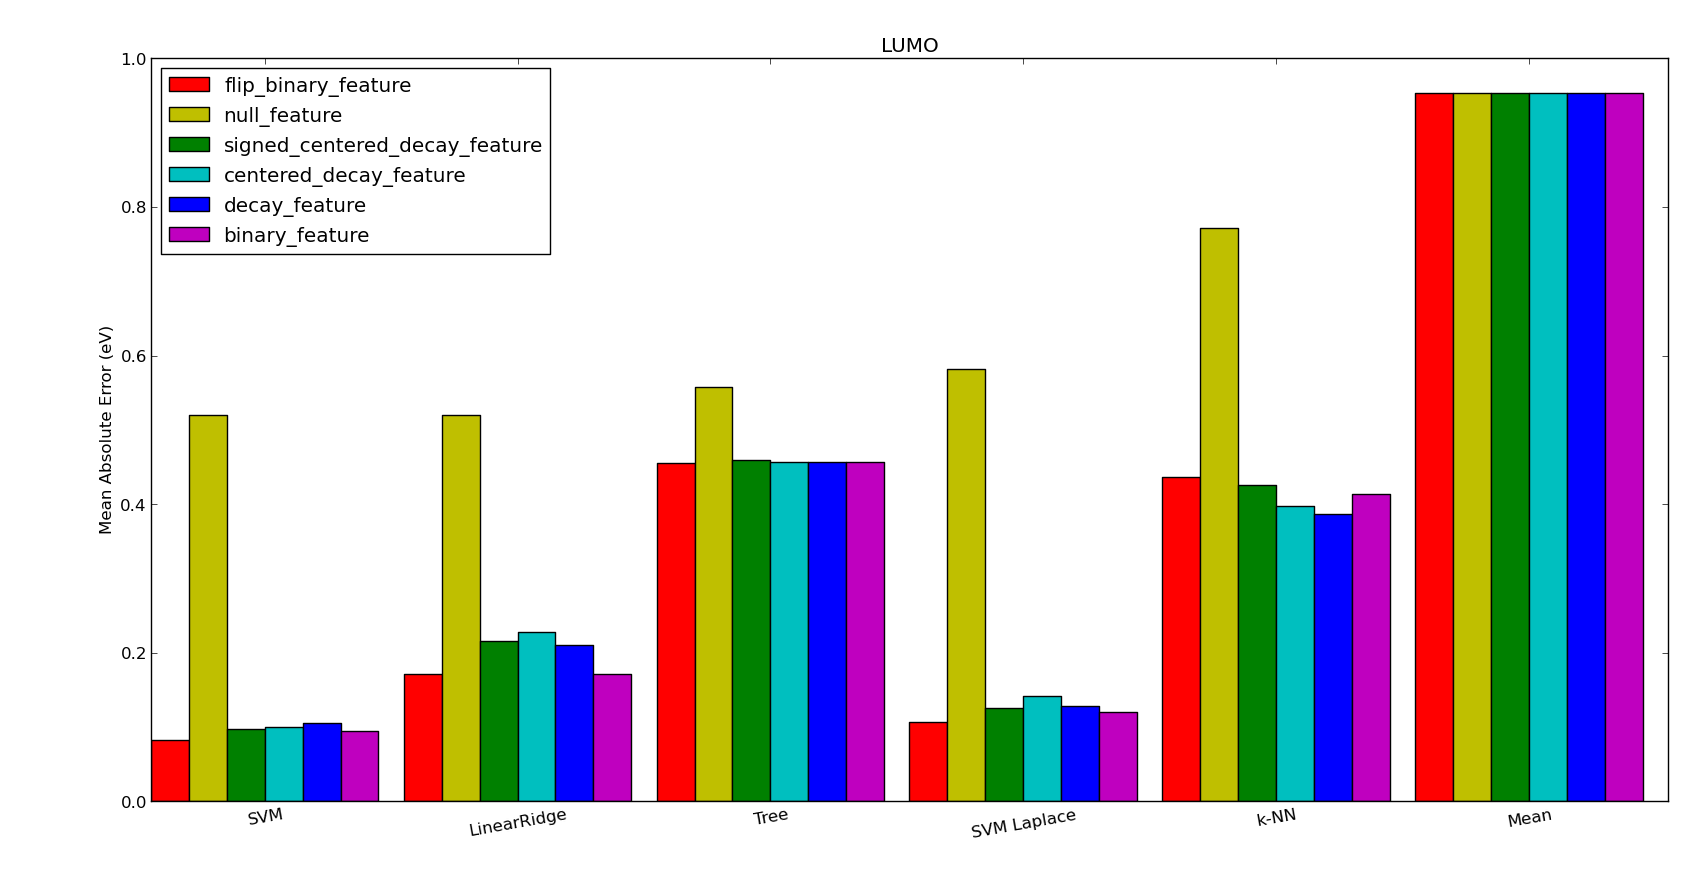
\includegraphics [width=1\textwidth]{lumo.png}
\caption{Test error results for LUMO}\label{fig2}
\end{center}
\end{figure}

\begin{figure}
\begin{center}
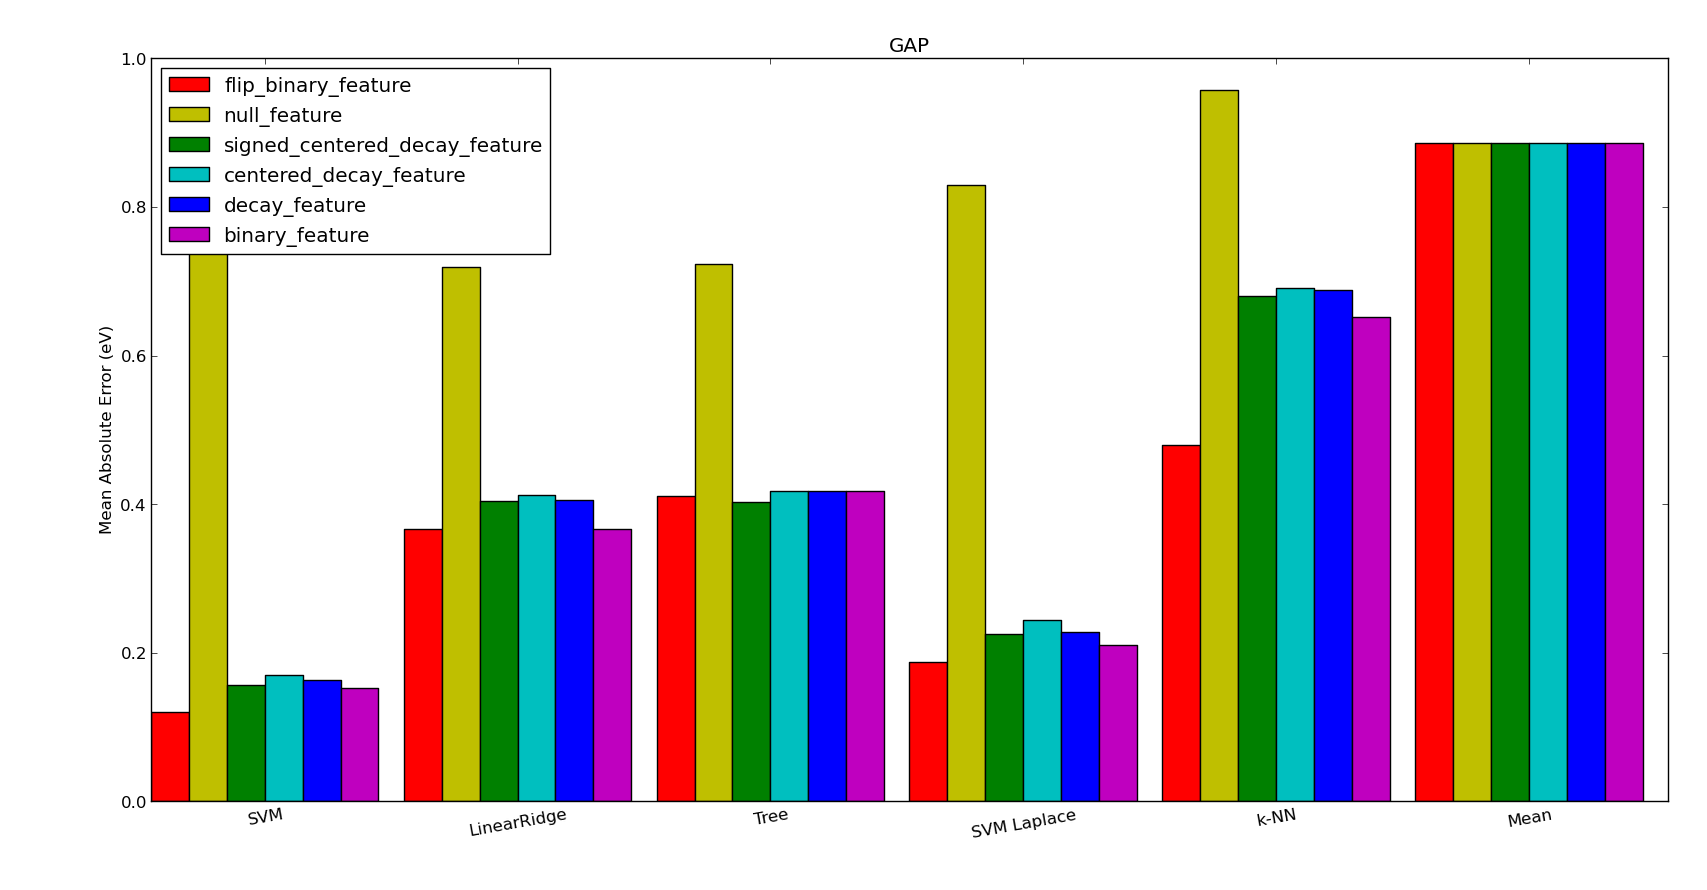
\includegraphics [width=1\textwidth]{gap.png}
\caption{Test error results for Band Gap}\label{fig3}
\end{center}
\end{figure}

These results show that machine learning algorithms run well on our feature vectors and predict reasonable values for HOMO, LUMO, and band gap. In all figures, the prediction errors from the five machine learning algorithms are well below the ``mean" method, indicating that these five methods work better than random guess. For a certain algorithm, prediction errors from flip binary feature, signed centered feature, centered decay feature, decay feature and binary feature are all significantly lower than null feature, which shows that our feature extraction also works better than just making predictions based on which dataset the structure came from.


It is also clear that errors from SVM (specifically with a Gaussian kernel) are lower than those from other models and reach the best prediction error so far, with errors hovering around 0.1 eV for the HOMO, LUMO, and 0.12 eV for the band gap. Overall, the error for the LUMO is slightly lower than the other two, but this can be accounted for if you take its value relative to the ``mean" method. The band gap has the highest error, this is assumed to be because the band gap is a much harder value to predict chemically (compared to the HOMO and LUMO). 

The different feature vectors do not seem to have a significant affect on the final errors for any of the methods, with the exception of the k-NN model, which seems to have more of a dependence on the feature vector. k-NN can also be seen to be the worst performing method (more recent work indicates that the high errors for k-NN and the tree regression are due to a bug in the code).

Overall, the flip binary feature vector has the best performance of all the feature vectors. This can be attributed to two factors, 1) it contains more relevant information than the binary feature, so it will quite readily out perform it. 2) This implies that the decay function used in the decay feature vectors is not a good representation of the physical relation between the structures.

\section{Next Steps and Goals}


% \textbf{Data Set}: We have constructed 557 structures and calculated their chemical properties, LUMO, HOMO and band gap, with three different methods. Altogether, there are 12 sets of data or 6694 data points. Based on the geometry and constituents of each structure, we have developed 6 different types of feature vectors including a null feature for comparison.


% \textbf{First Step and Evaluation}: Our first step is to characterize chemical structures such that they could be used for machine learning. We manage to characterize the chemical structures by transforming our data sets into 6 types of feature vectors. Furthermore, we have employed linear ridge regression, SVM, k-NN and regression tree along with our feature vectors and made a few predictions. The prediction errors are significantly lower than random guess, and lowest errors our models predict so far come from SVM together with decay feature, HOMO: 0.18 eV, LUMO: 0.13 eV, band gap: 0.24 eV. We have completed the first step and are now able to predict molecular properties predictions with our features and models.

\textbf{Feature Engineering} \\
HL is currently working on constructing new types of feature vectors based on SEQC calculations. As we mentioned before, these methods scale as $O(n^2)$ so even a series of calculations can be done in seconds for each of the molecules, but they give only qualitatively correct HOMO/LUMO/band gap values. Yet, it has been shown that combinations of cheap methods are able to lower the error to a level that is comparable to that of expensive methods\cite{hc}. HL has performed SEQC calculations with \textit{Gaussian} package on all of our current training/testing molecules and has done feature extraction using CC's file parser, and is going to evaluate the performance of this new type of feature vector.

\textbf{Machine Learning Algorithms} \\
ZL is working on SVM with kernel combinations. By so far our best result is achieved by SVM; there is for sure a good reason to continuously exploit its potential. He has designed and implemented various types of custom-defined kernel functions, and is going to test their performance.

CC is working on neural network algorithms. Based on his past experience with machine learning, he believes that neural network is a more general form, and is potentially the best choice. He has implemented gateway routines of neural network algorithms and has achieved low test errors just like what is seen with SVM with a Gaussian kernel.

\textbf{Data and Analysis} \\
CC is working on expanding our data sets to include more structures with Nitrogens. CC is also working on methods to better visualize the the dataset (specifically with being able to troubleshoot the neural networks).



Since band gap errors are usually larger than HOMO and LUMO errors, our minimum goal for this project is to drop the final prediction errors for HOMO and LUMO down below 0.1 eV, and prediction errors for band gap down below to 0.15 eV based on our data sets. For long term goal, we hope our method can be applied to every class of chemicals and predict their properties within the error limits stated above.

\nocite{Hansen}
\bibliography{interim}
\end{document}  
